\chapter{Les ventes}

\section{Page principale des ventes}

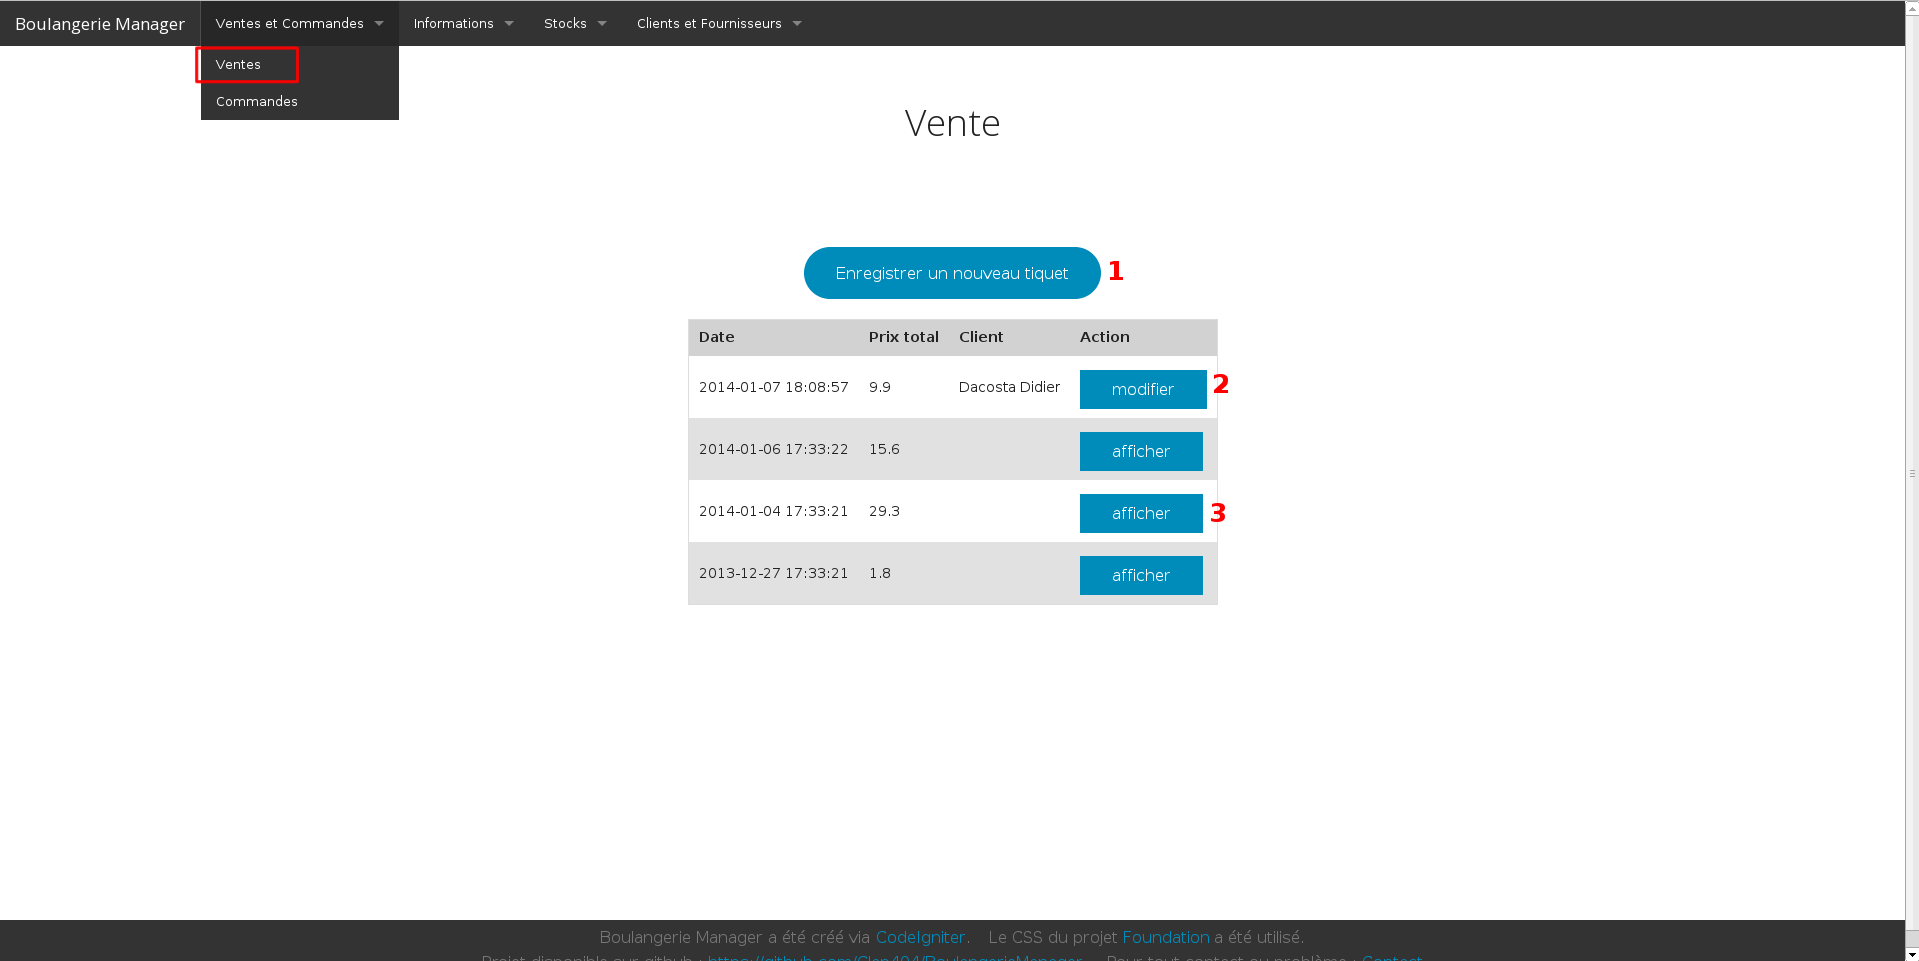
\includegraphics[scale=0.30]{vente1.png}

\paragraph{} Voici la page principale des ventes. Vous pouvez y accéder grâce à
l'onglet Ventes présent dans le menu Ventes et Commandes. Cette page vous donne
des informations à propos des ventes effectuées telles que la date, le prix
total et le client (si jamais il y en a un).

\paragraph{} Depuis cette page vous pouvez effectuer 3 actions différentes :
\begin{enumerate} 
    \item Enregistrer un nouveau ticket (voir section 2.2) 
    \item Modifier une vente, cette option n'est disponible que pour les ventes
    du jour (voir section 2.3) 
    \item Afficher une vente (voir section 2.3) 
\end{enumerate}

\section{Enregistrer un nouveau ticket}

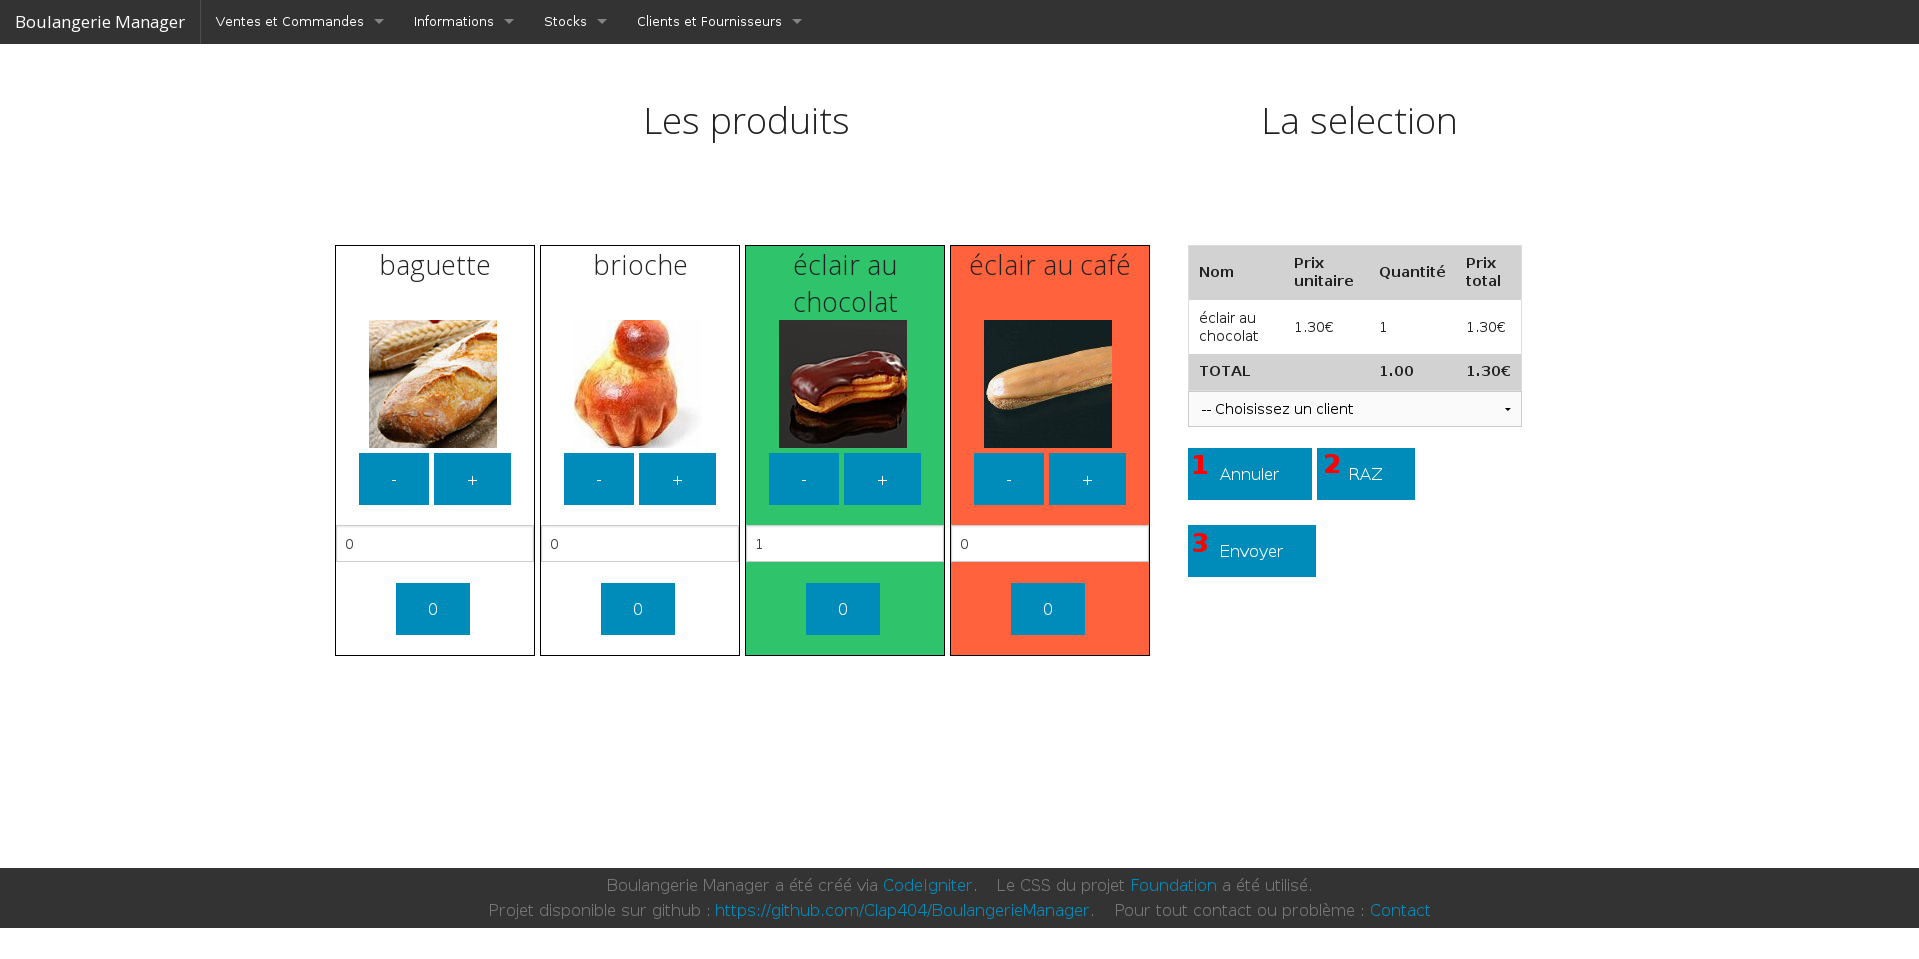
\includegraphics[scale=0.30]{vente2.png}

\paragraph{} Cette page vous servira à enregistrer un nouveau ticket de vente.
Les produits apparaissent sous forme d'une vignette. Chaque vignette contient
le nom du produit, une image du produit, un bouton moins et un bouton plus qui
servent respectivement à ajouter ou a enlever une unité du produit du ticket de
vente, un champs quantité qui vous permet d'ajouter le nombre choisi de ce
produit et un bouton 0 qui permet d'enlever ce produit du ticket de vente. Les
produits qui apparaissent en vert sont ceux ajoutés sur le ticket de vente. Les
produit qui apparaissent en rouge sont les produits indisponibles (tous vendus
ou non produits).

\paragraph{}
Le ticket de vente s'affiche sur le côté droit de l'écran. Il liste pour chaque
produit son prix unitaire, la quantité et le prix total. Il affiche également
la quantité totale et le prix total tous produits confondus. Vous pouvez
également attribuer le ticket à un client si ce dernier à été ajouté (voir
partie Client). 

\paragraph{}
Les trois boutons présents sous le ticket de vente vous permettent de :
\begin{enumerate}
    \item \textbf{Annuler} : revenir à la page principale des commandes sans
        valider cette dernière.
    \item \textbf{RAZ} : remettre à zero le ticket de vente.
    \item \textbf{Envoyer} : valider le ticket et le sauvegarder.
\end{enumerate}

\section{Modifier une vente}

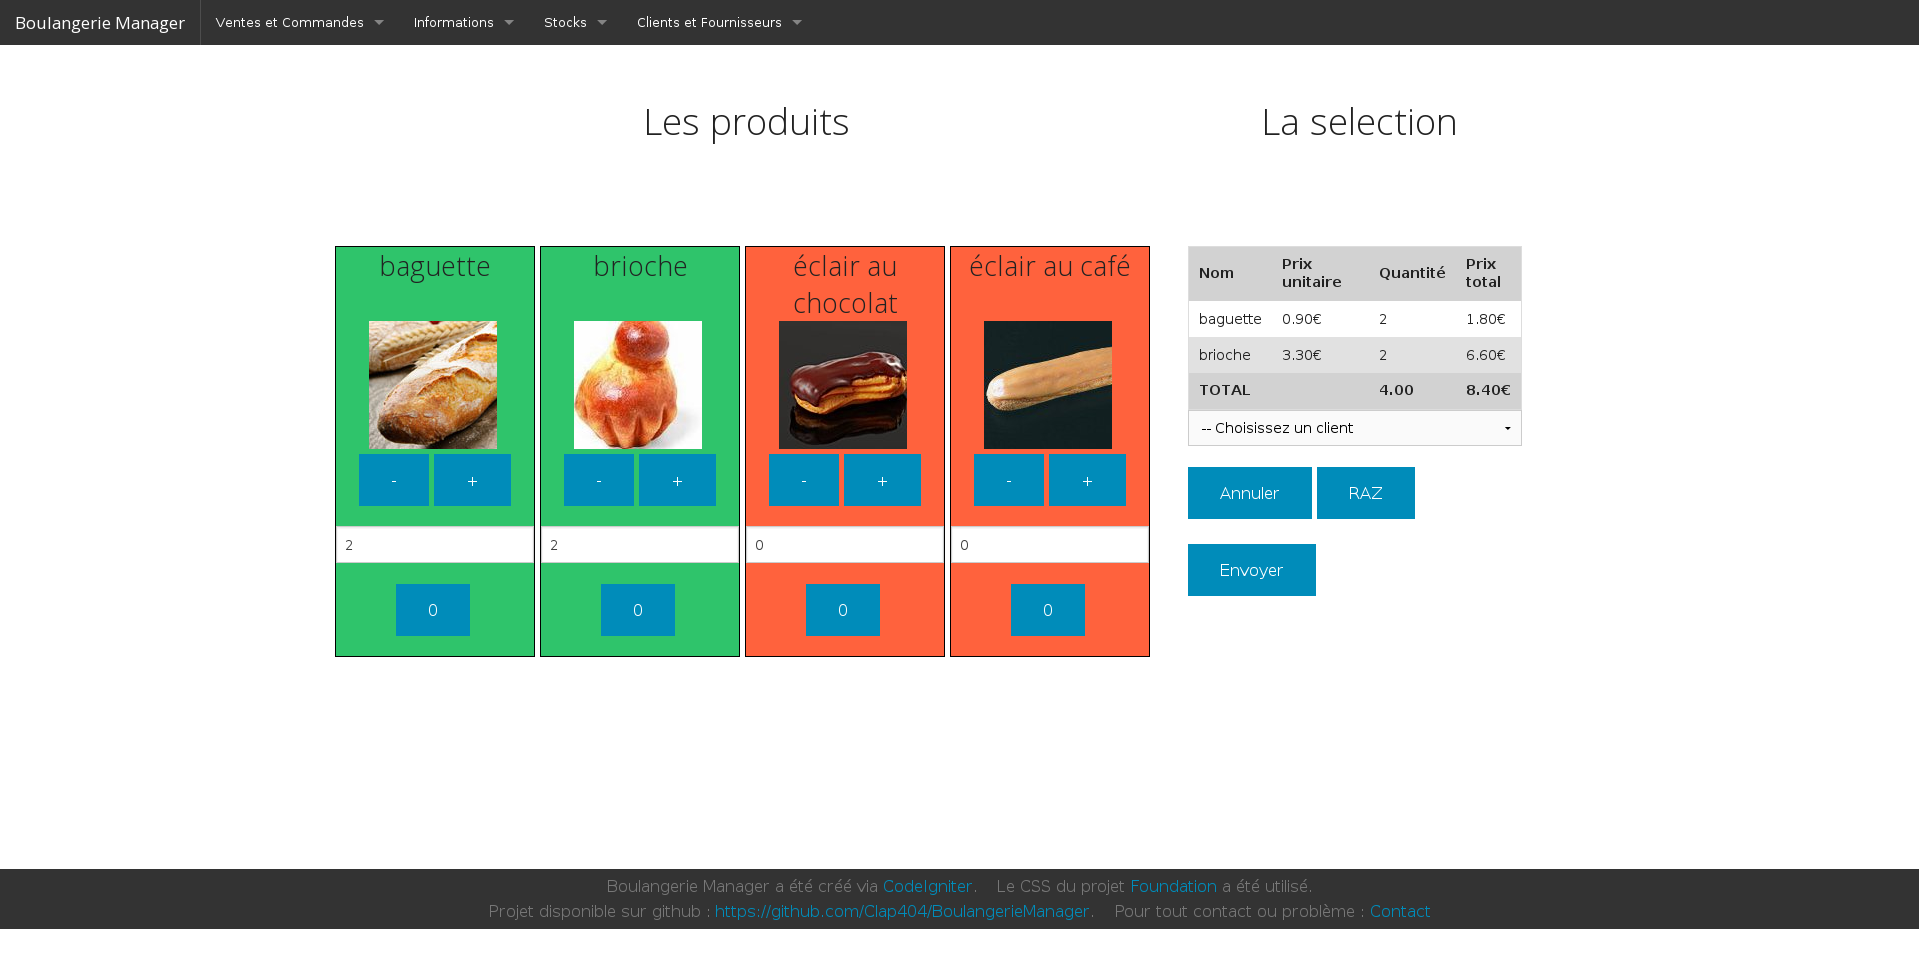
\includegraphics[scale=0.30]{vente3.png}

\paragraph{}
La page de modification des ventes est en tout point identique décris à la page décrite en 2.1. Elle vous permet de modifier une vente en ajoutant ou en retirant des produits et en ajoutant, modifiant, ou retirant un client attribué à cette vente.

\section{Afficher une vente}

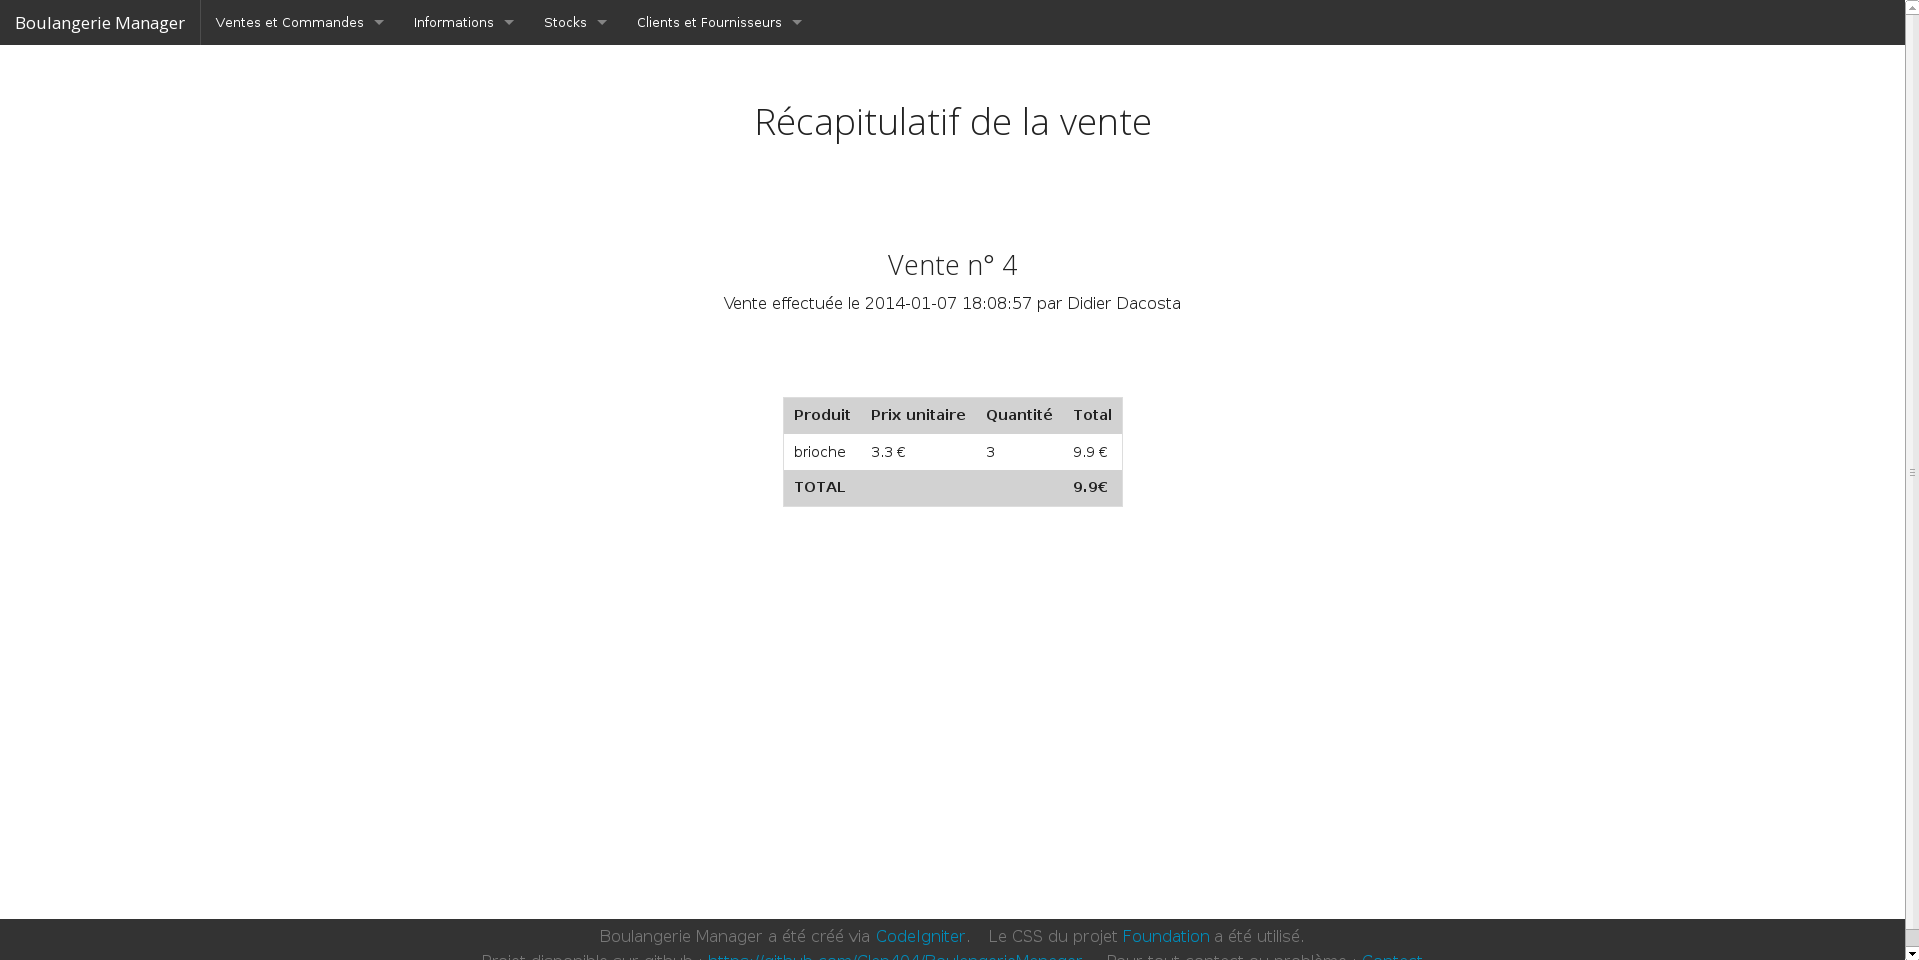
\includegraphics[scale=0.30]{vente4.png}

\paragraph{}
Cette page affiche les détails d'une vente. Elle récapitule les informations suivantes : 
\begin{itemize}
    \item La date de la vente
    \item Le client (s'il a été défini)
    \item Les produits vendus
    \item Le prix total
\end{itemize}
